\section{Metoda Newtona-Raphsona}
%%%%%%%%%%%%%%%%
\begin{frame}{Metoda Newtona-Raphsona}
	$f(x) = 0$, $\alpha$ - prosty pierwiastek\linebreak
	$x_{i-1}$ - przybliżenie $\alpha$\linebreak
	niech $\alpha = x_{i-1} + h$
	\[
		f(\alpha) = 0 = f(x_{i-1} + h) = f(x_{i-1}) + h \cdot f'(x_{i-1}) + \underbrace{\cdots}_{\text{pomijamy}}
	\]
	\[
		h = - \frac{f(x_{i-1})}{f'(x_{i-1})}
	\]
	\[
		\fbox{ $x_{i} = x_{i-1} - \frac{f(x_{i-1})}{f'(x_{i-1})}$ }
	\]
%	\[
	%	\left. \begin{array}{ll}
	%		f(x)\\
	%		f'(x)
	%	\end{array}\right\}
%	\]
\end{frame}
%%%%%%%%%%%%%%%%
\begin{frame}{Metoda Newtona-Raphsona}
	\centering
	\includegraphics[width=.7\linewidth]{img/7/7_4_1}
\end{frame}
%%%%%%%%%%%%%%%%
\begin{frame}{Metoda Newtona-Raphsona}
	\[
		\frac{f(x_{i-1})}{h} = \tan(\theta) = f'(x_{i-1})
	\]
	wzór iteracyjny:
	$x = \phi(x)$, czyli $\rightarrow$ $\phi(x) = x - \frac{f(x)}{f'(x)}$\linebreak
	
	\textbf{Warunek zbieżności: } $\phi'(x) = \frac{f''(x) \cdot f(x)}{(f'(x))^{2}}$ dla $x = \alpha$ : $f'(\alpha) \neq 0$, $\phi'(\alpha) = 0$ bo $f(\alpha) = 0$\linebreak
	
	Powinno istnieć otoczenie $\alpha$, w którym $\lvert \phi'(x) \rvert < 1$ tj. przy odpowiednim doborze $x_{0}$ met. N-R jest zawsze zbieżna do $\alpha$
\end{frame}

%%%%%%%%%%%%%%%%
\subsection{Twierdzenie o wyborze przedziału dla m. N-R}
\begin{frame}{Twierdzenie o wyborze przedziału dla m. N-R}
	Jeżeli: $I = \left[a, b\right]$ w którym:
	\begin{enumerate}
		\item $f(a) \cdot f(b) < 0$ - jest min. 1 pierwiastek
		\item $f'(x) \neq 0$, $x \in I$ - pierwiastek 1-krotny
		\item $f''(x) \geq 0$ lub $f''(x) \leq 0$ dla wszystkich $x \in I$\\
			(convex - wypukła) (concave = wklęsła)
		\item $\lvert \frac{f(a)}{f'(a)} \rvert < (b - a)$ i $\lvert \frac{f(b)}{f'(b)} \rvert < (b - a)$ - styczna przecina oś $x$  w  $I$
	\end{enumerate}
	to:
	metoda N-R jest zbieżna dla dowolnego $x_{0} \in I$ do $\alpha$
\end{frame}
\begin{frame}{Geometryczna interpretacja}
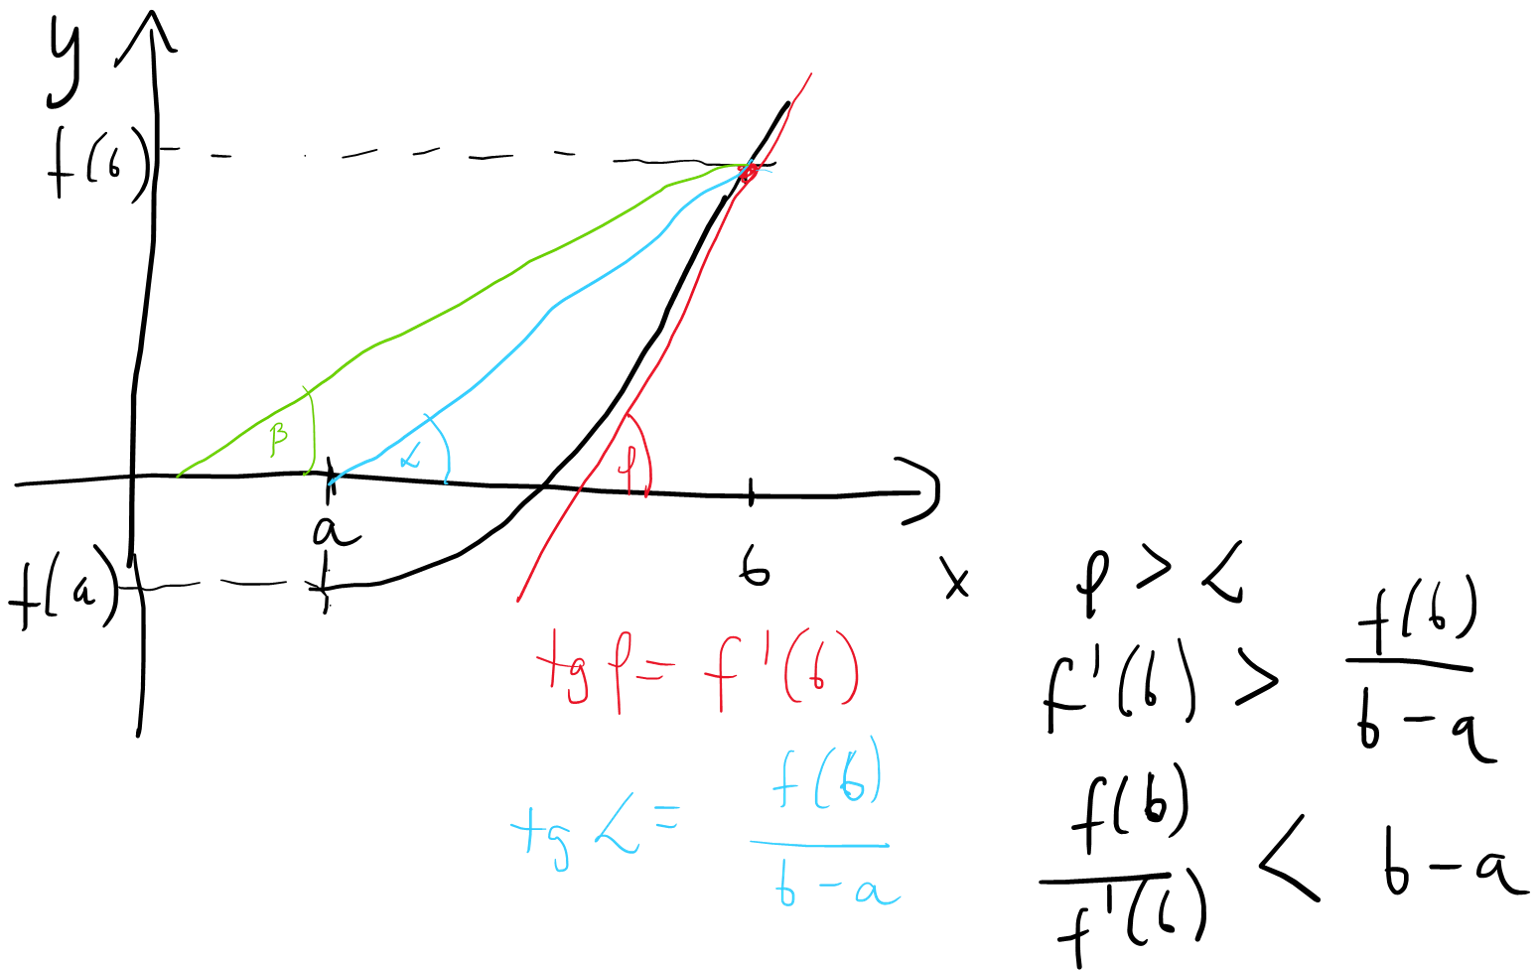
\includegraphics[width=0.9\textwidth]{img/7/nieliniowe1.png}
\end{frame}

%%%%%%%%%%%%%%%%
\subsection{Rząd zbieżności metody N-R}
\begin{frame}{Rząd zbieżności metody N-R}
	\begin{tabbing}
		\qquad\qquad \= $\phi(x) = x - \frac{f(x)}{f'(x)}$\\\\
		\> $\phi'(x) = \frac{f(x) \cdot f''(x)}{(f'(x))^{2}}; \quad \phi'(\alpha) = 0$\\\\
		\> $\phi''(x) = \frac{f'(x) \cdot f''(x)}{(f'(x))^{2}}+f(x) \cdot(\frac{f''(x)}{(f'(x))^{2}})' ; \quad \phi''(\alpha) \neq 0$ \quad \\
	\end{tabbing}
	- tylko pierwsza pochodna jest równa 0, więc mamy 2gi rząd tzn: $\epsilon_{i} \sim \epsilon_{i-1}^{2}$ błąd maleje kwadratowo z ilością iteracji
\end{frame}
%%%%%%%%%%%%%%%%
%\subsection{Dla m-krotnego %pierwiastka}
%\begin{frame}{Dla m-krotnego %pierwiastka}
%	\[
%		\fbox{$x_{i} = x_{i-1} - m \cdot \frac{f(x)}{f'(x)}$}
%	\]
%%	- też o zbieżności %kwadratowej 
%\end{frame}
%%%%%%%%%%%%%%%%
\subsection{Warunek zakończenia dla m. N-R}
\begin{frame}{Warunek zakończenia dla m. N-R}
	w procedurach bibliotecznych - \textbf{rozbudowane zabezpieczenia wyznaczanie:}\linebreak\linebreak
	- $\frac{\lvert x_{i} - x_{i-1} \rvert}{\lvert x_{i} \rvert}$\linebreak\linebreak
	- $\lvert f(x_{i}) \rvert$\linebreak\linebreak
	-ustalona maksymalna liczba iteracji
	%- $\lvert f'(x_{i}) \rvert$ - zbyt mały - to może:\linebreak\linebreak
\end{frame}
%%%%%%%%%%%%%%%%
\begin{frame}{Warunek zakończenia dla m. N-R}
	\textbf{Niebezpieczeństwa:}\linebreak
	\begin{columns}
		\column{.6\linewidth}
		\centering   \includegraphics[width=.7\linewidth]{img/7/7_4_2}
		\column{.6\linewidth}
		\includegraphics[width=.7\linewidth]{img/7/7_4_3}
	\end{columns}
	a) lokalne ekstrema\linebreak
	b) rozbieżny cykl iteracji %możliwe gdy f - wynik interpolacji $\Rightarrow$ inne $x_{0}$ 
	\linebreak często stosowana kombinacja: bisekcja (gdy kłopoty) + N-R
\end{frame}